\subsection{Discussion}

\begin{figure}
\center
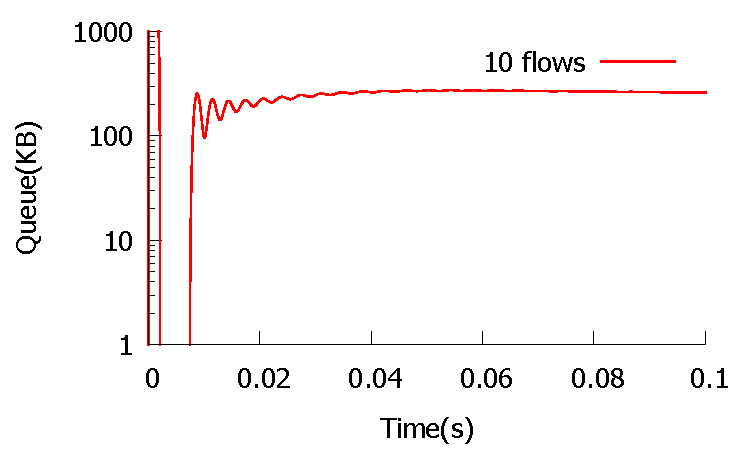
\includegraphics[width=0.33\textwidth]{figures/stable_q_85_pi.pdf}
\caption{PI marking scheme can stabilize DCQCN}
\label{fig:dcqcn_pi}
\end{figure}

\para{Using PI controller for enhanced stability:}
A more principled appraoch to stabilizing DCQCN for all operating regimes is to
use a PI~\cite{Hollot:PIController}-based packet marking scheme, instead of the
RED-like marking scheme of Equation (\ref{eq:mark}). We are currently
investigating this option in more detail; a sample result is shown in
Figure~\ref{fig:dcqcn_pi}. One important advantage of the using the PI
controller is that the staedy-state queue length is indepedent of the number of
flows.

\begin{figure}[t]
\center
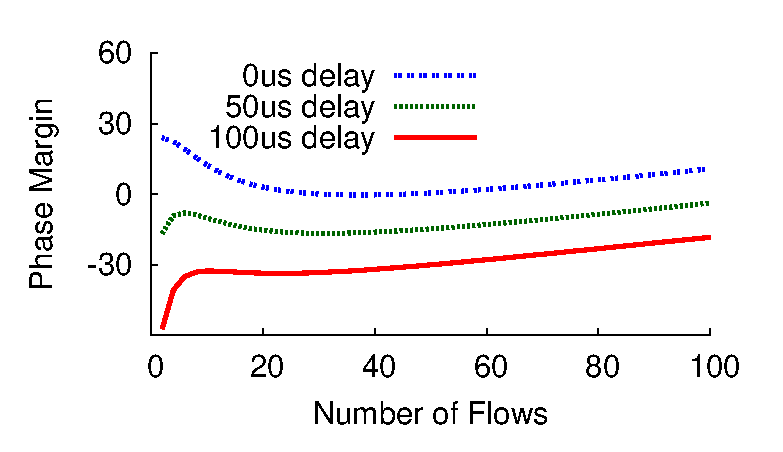
\includegraphics[width=0.33\textwidth]{figures/dcqcn_stability_100gbps.eps}
\caption{DCQCN stability with 100Gbps}
\end{figure}

\para{Extending to 100Gbps network.}  As the datacenter network fabric is moving
towards 100Gbps bandwidth, we analyze DCQCN stability given $C=100Gbps$. As
shown in Figure~\ref{fig:dcqcn_100gbps}, the default parameters of DCQCN work
reasonably well when the delay is small, {\em e.g.,} close to $0\mu s$.
However, DCQCN on 100Gbps is sensitive to the control loop delay. With
$50\mu s$ and $100\mu s$, the phase marginal decreases much more than in 40Gbps
case and leads to consistent instability.  The methods that stabilize the 40Gbps
system, like tuning down $R_{AI}$ and tuning up $K_{max}$, are also effective in
100Gbps system. Though we verified that tuning $R_{AI}$ and $K_{max}$
can help stabilize DCQCN at 100Gbps at the price of convergence speed and queue length, 
we believe PI controller is a more favorable option.

%DCQCN is stable at 100Gbps even when the control loop delay is $100\mu s$. TODO:
%similar for the PI controller. We conclude that DCQCN easily adapts to higher
%bandwidth fabrics with minor tunings. 

